\PassOptionsToPackage{table}{xcolor}
\documentclass[9pt,xcolor=x11names,compress]{beamer}

%% General document %%%%%%%%%%%%%%%%%%%%%%%%%%%%%%%%%%
\usepackage{graphicx}
\usepackage{tikz}
\usetikzlibrary{decorations.fractals,lindenmayersystems}
\usepackage{wasysym}
%%%%%%%%%%%%%%%%%%%%%%%%%%%%%%%%%%%%%%%%%%%%%%%%%%%%%%


%% Beamer Layout %%%%%%%%%%%%%%%%%%%%%%%%%%%%%%%%%%
\useoutertheme[subsection=false,shadow]{miniframes}
\useinnertheme{default}
\usefonttheme{serif}
\usepackage{palatino}

\setbeamerfont{title like}{shape=\scshape}
\setbeamerfont{frametitle}{shape=\scshape}

\setbeamercolor*{lower separation line head}{bg=DeepSkyBlue4} 
\setbeamercolor*{normal text}{fg=black,bg=white} 
\setbeamercolor*{alerted text}{fg=DeepSkyBlue4} 
\setbeamercolor*{example text}{fg=black} 
\setbeamercolor*{structure}{fg=black} 
 
\setbeamercolor*{palette tertiary}{fg=black,bg=black!10} 
\setbeamercolor*{palette quaternary}{fg=black,bg=black!10} 

\setbeamertemplate{blocks}[rounded][shadow=true]
\setbeamercolor{block title}{bg=DeepSkyBlue4}
\setbeamercolor{block title example}{bg=DeepSkyBlue4}
\setbeamercolor{block body}{bg=black!15!white}
\setbeamercolor{block body example}{bg=black!15!white}

\setbeamertemplate{navigation symbols}{}
%%%%%%%%%%%%%%%%%%%%%%%%%%%%%%%%%%%%%%%%%%%%%%%%%%

\title{Lesson 3: Relative Change.  Applications to Economics}
\author[Francisco Blanco-Silva]{Francisco Blanco-Silva}
\institute[USC]{University of South Carolina}
\date{
	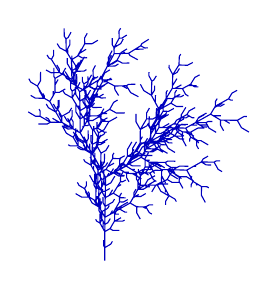
\begin{tikzpicture} 
    \draw [blue!75!black, rotate=90]
    [l-system={rule set={F -> FF-[-F+F]+[+F-F]}, axiom=F, order=4, step=2pt, 
        randomize step percent=25, angle=30, randomize angle percent=5}]
    lindenmayer system; 
	\end{tikzpicture}
}

\begin{document}

\frame{\titlepage}

\section{What do we know?}
\subsection{}

\begin{frame}[t]
\frametitle{What do we know?}
\framesubtitle{The General Program}
\begin{columns}[T]
\begin{column}{0.6\linewidth}
\begin{itemize}
\item Functions
\begin{itemize}
\item $x-$ and $y-$\alert{intercepts} ($f(x)=0$, $f(0)$)
\item \alert{Change} from $x=a$ to $x=b$ 
\begin{equation*}
	\Delta y = f(b)-f(a)
\end{equation*}
\item \alert{Average Rate of Change} from $x=a$ to $x=b$
\begin{equation*}
ARC=\frac{\Delta y}{\Delta x}=\frac{f(b)-f(a)}{b-a} 
\end{equation*}
\end{itemize}
\end{itemize}
\end{column}
\pause
\begin{column}{0.4\linewidth}
\begin{itemize}
	\item Kinds of functions:
	\begin{itemize}
		\item \alert{Linear} \\ $f(x)=a + mx$
	\end{itemize}
\end{itemize}
\end{column}
\end{columns}
\end{frame}

\section{Relative Change}
\subsection{}

\begin{frame}[c]
\frametitle{Relative Change}

Given a function $y=f(x)$, the \alert{relative change} between $x=a$ and $x=b$ is 
\begin{equation*}
RC=\frac{\Delta y}{f(a)}=\frac{f(b)-f(a)}{f(a)}.
\end{equation*}
It does not carry units.  Instead, if we multiply it by 100, we may express it as a percentage.
\end{frame}

\begin{frame}[t]\frametitle{Relative Change}

\framesubtitle{Examples}

\begin{example}
If the population increases by 1000 people, find the relative change in the population of:
\begin{itemize}
\item Coyote, NM (pop.~1,559)
\item NYC (pop.~8,250,000)
\end{itemize}
\end{example}
\uncover<2->{
For Coyote: $f(a)=1559, f(b)=1559+1000=2559$; therefore,
\begin{equation*}
\text{RC}=\frac{f(b)-f(a)}{f(a)}=\frac{1000}{1559} \approx 0.6414, \text{ an \alert{increase} of about } 64.14\%
\end{equation*}}
\uncover<3->{
	
	For NYC: 
	\begin{equation*}
	\text{RC} = \frac{1000}{8250000} \approx  0.00012, \text{ a (very small!) \alert{increase} of about } 0.012\%
	\end{equation*}	
}
\end{frame}

\begin{frame}[t]\frametitle{Relative Change}
    
\framesubtitle{Examples}

\begin{example}
Find the relative change in the price of a \$75.99 pair of jeans, if the sale price is \$52.99.
\end{example}
\begin{equation*}
\uncover<2->{\text{RC} = \frac{f(b) - f(a)}{f(a)}}\uncover<3->{= \frac{52.99 - 75.99}{75.99} = \frac{-23}{75.99} \approx -0.303}
\end{equation*}
\uncover<4->{The price has been \alert{reduced} by 30\% for this sale.}

\end{frame}

\section{Applications to Economics}
\subsection{}

\begin{frame}
\frametitle{Applications to Economics}
Some of the functions of interest to decision-making in a firm, industry of government are
\begin{itemize}
\item<1-> The \alert{Cost} function.
\begin{quotation}
$\text{Total Cost} = \text{Fixed Cost} + \text{Variable Cost}$
\end{quotation}
\item<2-> The \alert{Revenue} function.
\begin{quotation}
$\text{Revenue} = \text{Price} \times \text{Quantity}$
\end{quotation}
\item<3-> The \alert{Profit} function.
\begin{quotation}
$\text{Profit} = \text{Revenue} - \text{Cost}$
\end{quotation}
\item<4-> The \alert{Depreciation} function.
\item<5-> \alert{Supply} and \alert{Demand} curves. \alert{Equilibria}.
\end{itemize}
\end{frame}


\subsection{}

\begin{frame}
\frametitle{Cost, Revenue, Profit}
\framesubtitle{Examples}
\begin{example}[Making smartphones]
The factory and machinery needed to begin production are fixed costs, which are incurred even if no phones are made.  The cost of labor and materials are variable costs, since these quantities depend on how many are made.  The fixed costs for this company are \$24,000 and the variable costs are \$37 per phone. 
\begin{enumerate}
\item What is the Total Cost function for this company?
\item If phones sell for \$250 each, find the manufacturer's revenue function. 
\item Sketch these functions, and identify their $y-$intercept and slope.
\item Find a formula for the profit function of the smartphone manufacturer.  Find the \emph{break-even point}. 
\end{enumerate}
\end{example}
\end{frame}

\begin{frame}[t]
\frametitle{Cost, Revenue, Profit}
\framesubtitle{Examples}
\begin{enumerate}
\item<1-> $C=f(q) \uncover<2->{=\underbrace{24000}_{\text{fixed}}+\underbrace{37q}_{\text{variable}}}$

($q$ is the quantity, in number of items, $C$ is the total cost, in dollars)
\item<3-> The Revenue is $R=f(q)=250q$.  
\item<4-> The graph of the \alert{Cost function} is a line with slope $37$ and $y-$intercept $24,000$.  The graph of the \alert{Revenue function} is another line, with slope $250$ and $y-$intercept equal to zero.

\uncover<4->{
	
\begin{center}
\includegraphics[width=0.6\linewidth]{figure_1.png}
\end{center}

}
\end{enumerate}
\end{frame}

\begin{frame}[t]\frametitle{Cost, Revenue, Profit}
\framesubtitle{Examples}

\begin{enumerate}\addtocounter{enumi}{3}
\item<1-> The Profit is $\Pi=f(q)=\underbrace{250q}_{\text{Revenue}}-\underbrace{(24000+37q)}_{Cost} \uncover<2->{=213q-24000.}$  

\uncover<3->{The break-even point happens when Revenue equals Cost:
\begin{equation*}
250q = 24000+37q 
\end{equation*}
\begin{equation*}
\uncover<4->{q=\frac{24000}{213}\approx 112 \text{ cellphones}}
\end{equation*}}
\end{enumerate}
\end{frame}

\begin{frame}
\frametitle{Depreciation}
\framesubtitle{Examples}
\begin{example}
Suppose that the smartphone manufacturer has a machine that costs \$20,000 and is sold ten years later for \$3,000.  
\begin{quote}
\emph{We say that the value of the machine depreciates from \$20,000 to a resale value of \$3,000 in ten years}. 
\end{quote}
The depreciation formula gives the value $V=f(t)$ in dollars of the machine as a function of $t$ in years.  Assume that the value depreciates linearly.  Find that function.
\end{example}
\uncover<2->{
\textbf{Hint:} Find two points on this line by gathering info from the body of the problem: $(0,20000)$ is one, $(10,3000)$ is another. Note one is a $y-$intercept, and with the other you may compute the slope.  Use the slope-intercept equation of a line.}
\begin{equation*}
\uncover<3->{V=f(t)=20000-1700q}
\end{equation*}
\end{frame}

\begin{frame}\frametitle{Applications to Economics}
\framesubtitle{Supply and Demand}
The quantity of an item $q$ that is manufactured  and sold depends on its price.  Higher prices make manufacturers supply more, but consumers demand less.
\begin{itemize}
\item A \alert{supply curve} relates the quantity of items that manufacturers are willing to make compared to the \alert{price per unit}.
\item A \alert{demand curve} relates the quantity of items that buyers are willing to purchase compared to the \alert{price per unit}.
\item The \alert{equilibrium price and quantity}, $(p^\star, q^\star)$, is found where both curves cross.
\end{itemize}

\pause
\alert{Hint:} The higher the price, the more units would the manufacturer want to sell.  The lower the price, the more units would the buyer want to purchase!

\end{frame}

\begin{frame}
\frametitle{Supply and Demand}
\framesubtitle{Examples}
\begin{example}
One of the tables below represents a supply curve; the other represents a demand curve.
\begin{center}
\begin{tabular}{c||c|c|c|c|c|c|c|}
\hline
p & 182 & 167 & 153 & 143 & 133 & 125 & 118  \\
\hline
q & 5 & 10 & 15 & 20 & 25 & 30 & 35 \\
\hline
\end{tabular}

\vspace{0.5cm}
\begin{tabular}{c||c|c|c|c|c|c|c|}
\hline
p & 6 & 35 & 66 & 110 & 166 & 235 & 316  \\
\hline
q & 5 & 10 & 15 & 20 & 25 & 30 & 35 \\
\hline
\end{tabular}
\end{center}
\begin{itemize}
\item Which one is which? \uncover<2->{\alert{TOP: demand}}
\item At a price of \$155, approximately how many items would consumers purchase? \uncover<3->{\alert{between 10 and 15 items}}
\item What would the price have to be if you wanted consumers to buy at least 20 items? \uncover<4->{\alert{\$143}}
\end{itemize}
\end{example}
\end{frame}
\end{document}